\chapter[AM Detection with Automatic Gain Control]{AM Detection with Automatic Gain Control}
\label{agcdetect}
\section*{Aim}
To demodulate the message content from AM signal. Also detect the automatic gain control signal from the received AM signal.
\section*{Theory}


A simple AM demodulator is a diode envelope detector. It can be implemented by a simple diode envelope detector to eliminate the negative half of the carrier envelope followed by a simple RC filter to remove the high frequency carrier. The result will be the low frequency envelope which is the demodulated message.

A point contact diode with low junction capacitance is used in the circuit as it is has to rectify high frequency carrier. It offers low impedence at high frequency. The RC elements connected after the diode acts as a filter. It acts as a lowpass filter which eliminates high frequency carrier at the same time it retains the low frequency message signal. 

Thus the output of the filter contains the low fequency modulating signal with a dc offset. The dc offset voltage is proportional to the strength of the modulated signal received by the receiver in a transmission reception system, which inturn is proportional to the strength(amplitude) of the carrier. This dc value may be used for automatic gain control(AGC) of intermediate frequency(IF) amplifier stages. The Automatic gain control compensates for minor variations in the received RF signal level. The AGC circuit automatically increases the receiver gain for weak RF input levels and automatically decreases the receiver gain when strong RF signal is received\footnote{For detailed explanation, refer to Chapter 5 of \cite{Tomasi}}.
\paragraph{Simple AGC:} It is implemented in the form of a circuit which extracts the dc offset voltage which is present along with the demodulated message. This volatge is fed as degenerative or negtive feedback to the control the gain of superheterodyne receivers. 
\paragraph{Delayed AGC:}In simple AGC circuits even if the signal level received is low, the AGC circuit operates and the overall gain of the receiver gets reduced. To avoid this situation, a delayed AGC circuit is used. In this case AGC bias voltage is not applied to amplifiers, until signal strength has reached a predetermined level after which AGC bias is applied like simple AGC.

\section*{Design}

After the positive envelope detector, a properly designed low pass filter is added to filter out the high frequency carrier and to retain the low frequency modulating signal. This signal contains a dc level also which can be used for automatic Gain Control (AGC) for the IF amplifier stages of a superhetrodyne receiver.\\

\noindent Let the carrier frequency be $f_c=455\ kHz$ and maximum modulating signal frequency be $f_m=10\ kHz$

\noindent Inorder to design a lowpass filter with upper cutoff frequency 10 kHz,
\begin{equation}
f_H=\frac{1}{2\pi R_dC_d}
\end{equation}
\begin{equation}
10\ kHz=\frac{1}{2\pi R_dC_d}
\end{equation}
\noindent Select $C_d=\ 0.001 \mu F$. Then $R_d=\ 16.1k\Omega$.
Choose $R_d=\ 15k\Omega \ or\ 22k\Omega$ standard resistor values.\\

\noindent Make a $\pi$ filter (for better performance) using these $R_d$ and $C_d$ values. This completes the envelope detector part.
\paragraph{AGC Circuit:} The AGC lowpass filter $R_a$ and $C_a$ is seected in such a way as to eliminate full ac from the output and get a pure dc AGC voltage. 
Hence assuming a cutoff frequency of 10 Hz to eliminte the fluctuations,
\begin{equation}
10 Hz= \frac{1}{2\pi R_aC_a}
\end{equation}
\noindent Assuming $C_a=1 \mu F$, we get $R_a=22 k \Omega$

The actual modulating signal can be obtained by  filtering out the dc components using a high value caacitance like  $10\mu F$.

%\paragraph{Delayed AGC Circuit:}
%Here the simple AGC circuit is applied to a difference amplifier.  Delayed AGC output will be produced only when input voltage $V_i$ exceeds the threshold voltage which can be set to the desired value by adjusting the dc level of the potentiometer.
%
%LM 741 opamp is chosen as the amplifying element. It is configured in difference amplifier mode. The Simple AGC volatge derived from previous 
%circuit is used as the input to the inverting terminal of the  difference amplifier throgh the input resistance $R_i$. The threshold voltage is set at the non-inverting terminal. The voltage at non-inverting terminal can be varied in between +12V and 0V.
%
%The gain of the difference volatage is determined by the values of feedback resistance $R_f$, input resistance $R_i$ and the position of variabale terminal of the potentiometer. The opamap is biased using +12V and -12 V respectively. 
%The values of ristances are chosen as:

%\begin{equation}
%R_i\ =\ R_f\ =R_{pot}\ =100 k \Omega
%\end{equation}
\section*{Circuit Diagram}
The detector circuit with simple AGC is shown in Figure. \ref{detectagcckt}.%and with delayed AGC is shown in Fig. \ref{delayedagcckt}.
\begin{figure}

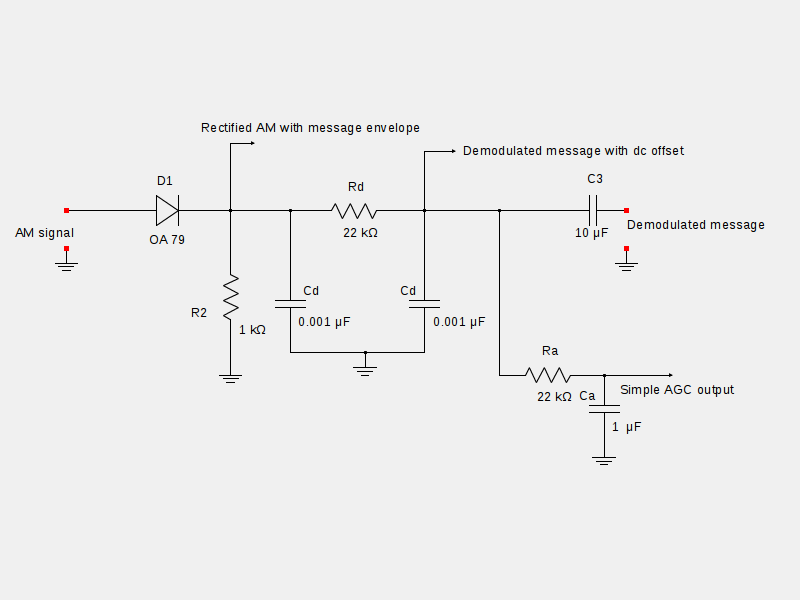
\includegraphics[height=8cm,width=15cm, trim=0cm 2cm 0cm 3cm,clip=true]{amdetectagc.png}
\caption{Detector circuit with Simple AGC}
\label{detectagcckt}
\end{figure}

%\begin{figure}
%
%\centering 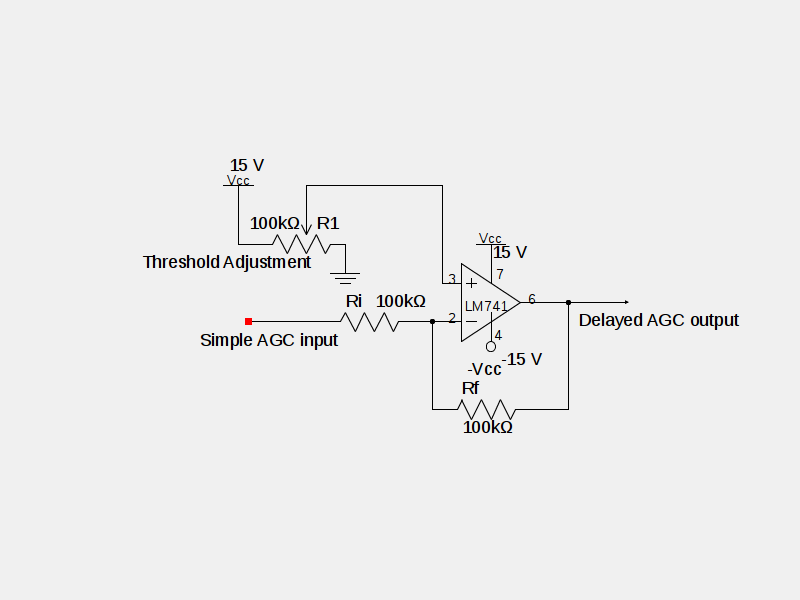
\includegraphics[height=8cm,width=12cm, trim=0cm 0cm 0cm 3cm,clip=true]{delayedagc.png}
%\caption{Detector circuit for delayed AGC}
%\label{delayedagcckt}
%\end{figure}
\section*{Procedure}
\begin{enumerate}
\item
Connect the diode to the output of AM signal(See Figure. \ref{amenv}) as in the circuit diagram Fig. \ref{detectagcckt}.
\item
Connect load resistance $R_L$ and observe the outputwaveform on a CRO and plot it.
\item
Connect the $\pi$ filter circuit of $R_d$ and $C_d$ and observe the output waveform on a CRO and plot it.
\item
Obtain the demodulated output without dc offset by connecting capacitor $C_3$. Observe it on a CRO and plot it.
\item
Connect the lowpass filter using $C_a$ and $R_a$ for obtaining AGC voltage level. Observe it on a CRO and plot it.
\item Vary the modulation index by changing carrier or modulating signal levels. Plot the simple AGC charateristics with modulation index on x-axis and AGC voltage level on y-axis.
\item
Eliminte the dc offset and observe the modulating signal from the $10\mu F$ capacitor as shown in the circuit diagram.
%\item
%Feed the AGC voltage to the delayed AGC	circuit of Fig. \ref{delayedagcckt}.
%\item
%Set the threshold to a fixed value, say $V_{threshold}=).5 V$. Keep the carier amplitude to the lowest, so that modulation index is 1.
%\item
%Slightly go on increasing the carrier amplitude. Note that for small values of carrier amplitude, delayed AGC voltage is positive. When it is above a certain limit the delayed AGC value becomes negative.
\end{enumerate}
\section*{Observation}
The following are the observed results of the experiment. See Figure. \ref{aminter} and Figure. \ref{demodagcwaves} for the waveforms of intermediate and final stages.
\begin{figure}
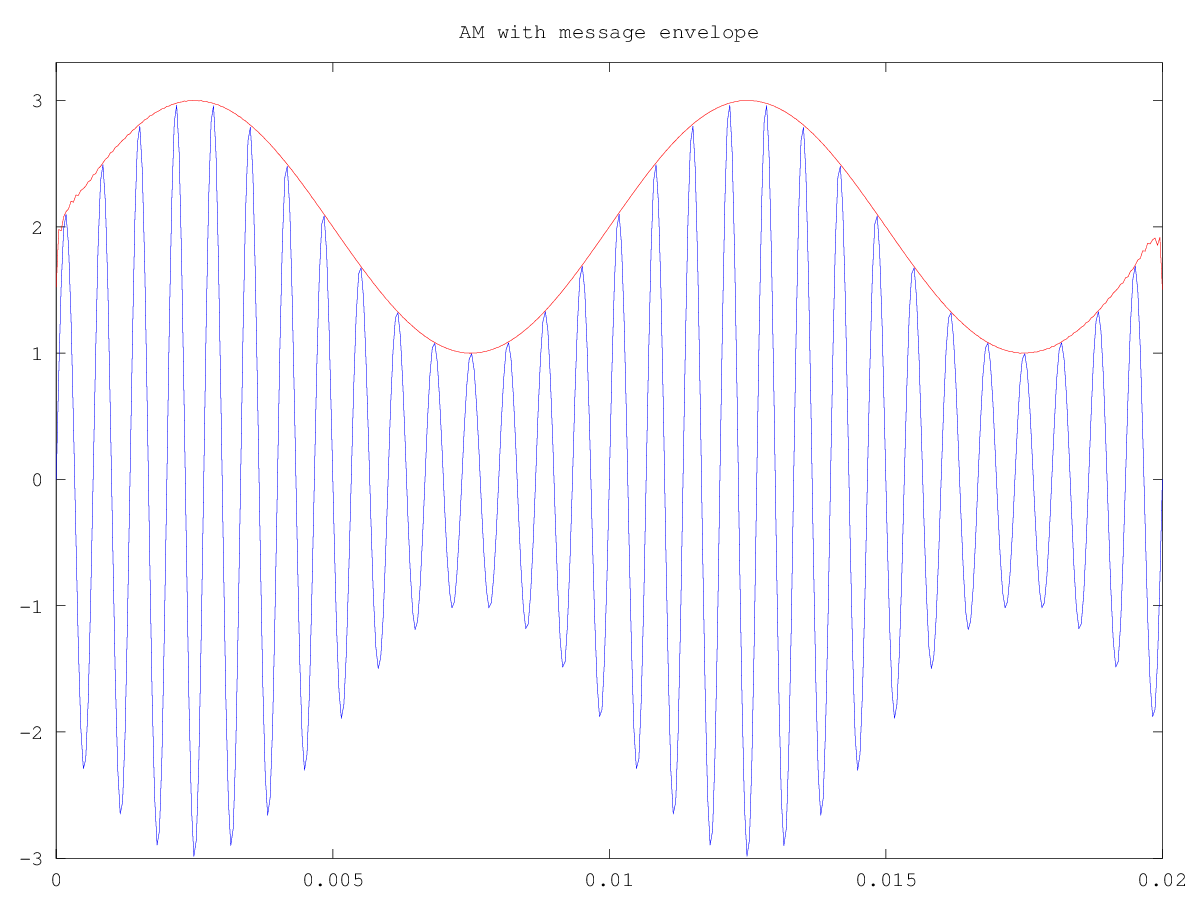
\includegraphics[height=8cm, width=12cm]{am.png}
\caption{AM with message envelope}
\label{amenv}
\end{figure}
\begin{figure}
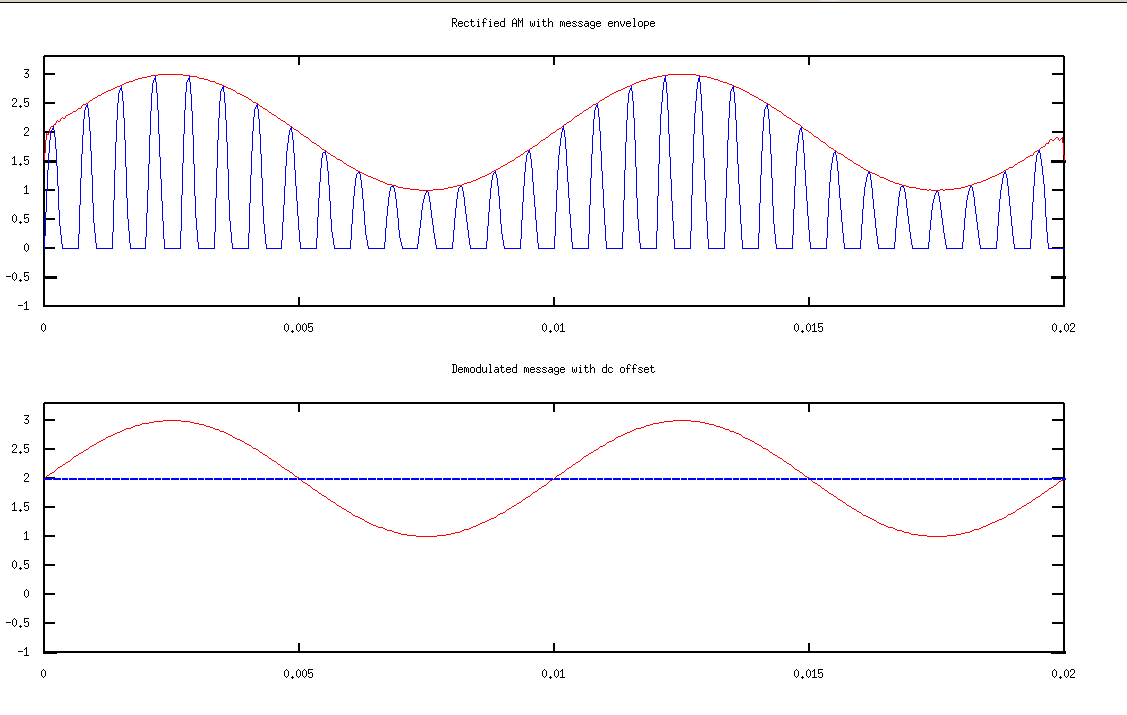
\includegraphics[height=8cm, width=12cm]{demodfig.png}
\caption{Intermediate stage of demodulation}
\label{aminter}

\end{figure}
\begin{figure}
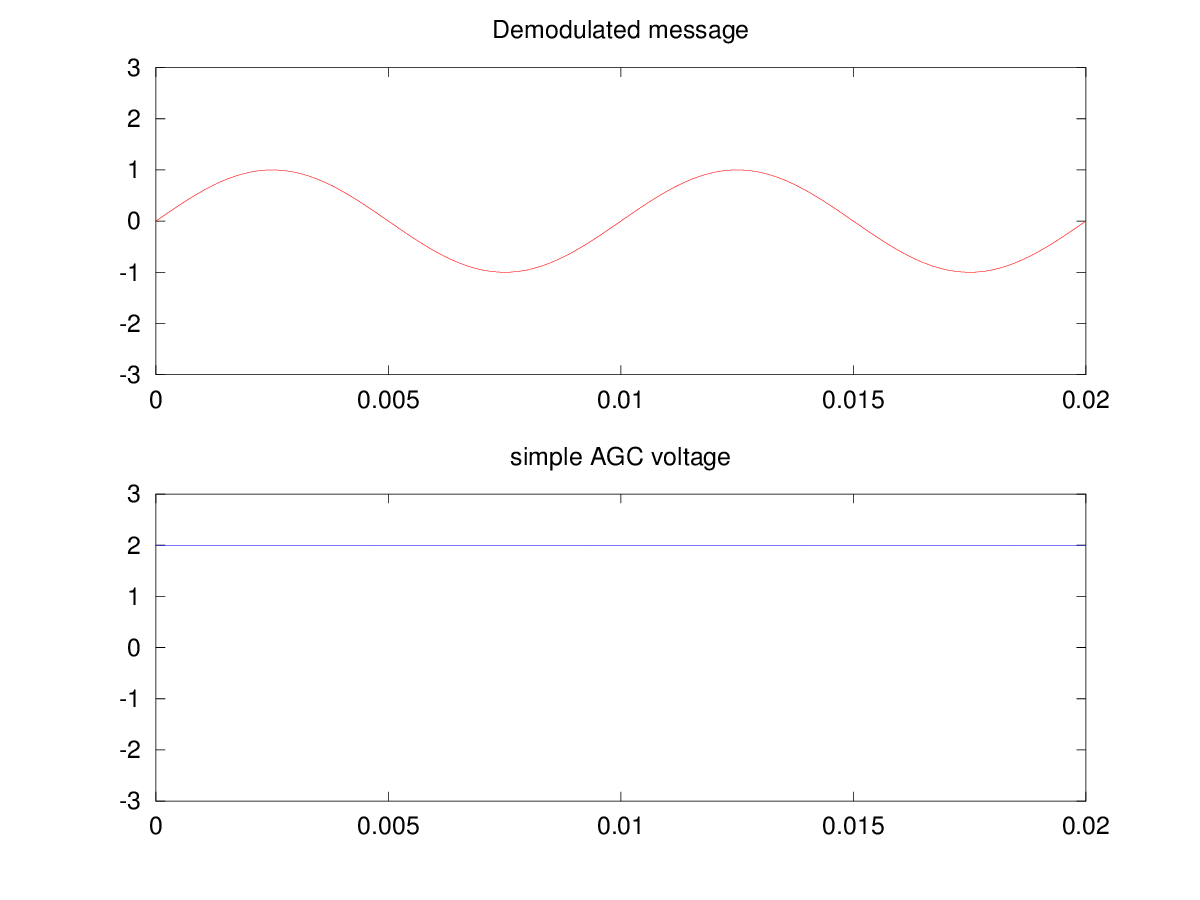
\includegraphics[height=8cm, width=\textwidth]{demodagc2.png}
\caption{Output waveforms from demodulation circuit}
\label{demodagcwaves}
\end{figure}

\section*{Result}

Demodulation circuit was designed and implemented with simple AGC.
